\chapter{Développement d'outils d'investigation}
\label{chap:2}
\section{Méthode de modélisation au niveau système}

Pésentation des différents composants modélisés

% Need to simulate from source to input for soft-failure analysis
In this chapter, a methodology for building electrical ESD models is proposed.
It enables simulation of waveforms from the ESD source to an integrated circuit pin.
This is a preliminary step for enabling simulation of soft-failures inside the chip.
The proposed methodology is modular and offers to reuse models between common devices found in ESD laboratories.
A typical ESD test setup comprises equipments such as DC sources, oscilloscopes, and stress generators.
Equipments are connected together with wires, coaxial cables, twisted wire pairs, etc.
The integrated circuit under test is often soldered onto a printed circuit board.
\gls{PCB}s usually host multiple kind of discrete devices, such as passive devices, ESD protections, common-mode chokes, relays, etc.
Components are connected together by metal tracks.
The goal of the proposed methodology is to build a library of all those elements, from lab equipments down to tiny discrete components.
Each model of the library will be qualified independently with individual characterization and comparison with its model.

% Assemble models together to build the complete thing
%TODO: Etoffer
After the library is constructed, models can be connected together to simulate the entire system.
The topology of the system serves as a blueprint for connecting models.

Présentation de la modélisation d'une TLINE ?

% Cables and delays identified as important for esd sims - because of similar order of magnitude
Cables are critial elements in any \gls{esd} test setup.
They introduce significant propagation delays in regard of the duration of an electrostatic discharge.
A 50\textOmega{} coaxial cable has a propagation ratio of approximately 5 ns/m.
In a laboratory, it is common to find cables of tens of centimers to a couple of meters long, resulting in delays between 1 ns and 10 ns.
As a comparison, the scale of an electrostatic discharge is a few hundred nanoseconds.
Both values are near the same order of magnitude and a large impact from cables on the simulation can logically be expected.
Cables, microstrip lines, wires and electrical propagation media behave as transmission lines.
Transmission lines were originally analysed by J. Maxwell, L. Kelvin and O. Heavyside and a huge amount of studies on the topic are available in the litterature \cite{branin-tl-ref, hf-coax,lossy-tl,emc-analysis-tl}.

% model delays with lossless TL
Transmission lines are characterized by their characteristic impedance, supposedly constant on the entire line.
It is determined by its cross-sectional dimensions and constituting materials.
For coaxial cables, common characteristic impedances are 50\textOmega{} or 75\textOmega{}.
This value is equivalent to the resistance that could be measured statically between outer and inner conductors for an \textbf{infinitely long} transmission line.
All transmission lines are lossy, meaning that some a part of the incoming power traversing it is dissipated.
In most cases though, losses are very small and negligible, and the line is considered lossless.
The behavior of the line is also frequency-dependant.
Losses, characteristic impedance and other properties can change above certain frequencies.
For frequencies below a GHz, most cables and metal strips can be correctly approximated by a lossless and non frequency-dependant line.

% Distributed model
The most popular line model in the ESD field is based on lumped capacitance and inductance.
The model is a series of lumped L-C networks as illustrated in Fig. \ref{fig:dis-line-model}.
Values for the element can be computed from the characteristic impedance \gls{Zc} with Eq. \ref{eq:characteristic-impedance}.

\begin{figure}[!h]
  \centering
  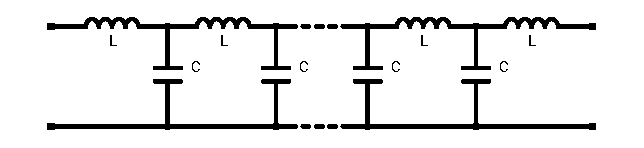
\includegraphics[width=0.7\textwidth]{src/2/figures/lc_ladder.pdf}
  \caption{Electrical distributed LC ladder model of a lossless transmission line}
  \label{fig:dis-line-model}
\end{figure}

% Perks and disavantages
The distributed model supports easily lossy transmission lines by adding a unit resistance or conductance between signal and ground, or in series with the signal.
On the other hand, this model does not scale well as cables get longer.
To keep the same bandwidth with a longer cable, the only solution is to increase the element count, resulting in longer simulation time.
Also, this model will always be bandwidth limited, otherwise it would require an infinite amount of infinitely small elements.


% Behavioral model
The two-port network model described by H. Branin \cite{branin-tl-ref} is a much better alternative to the distributed model.
It can describe efficiently and with great accuracy the behavior of uniform lossless transmission lines.
The model is constituted of two voltage-controlled voltage sources and two resistors (Fig. \ref{fig:beh-line-model}).
Compared to the distributed model, the behavioral model has by design an infinite bandwith, and is extremely fast to simulate.
It also is constant in complexity, because the simulation time is independant of the cable's delay or required bandwidth

\begin{figure}[!h]
  \centering
  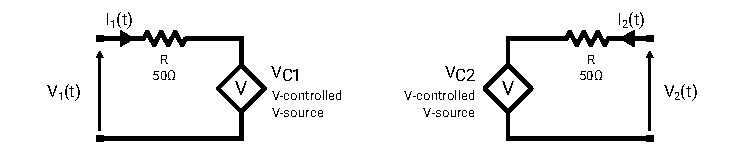
\includegraphics[width=\textwidth]{src/2/figures/behavioral_line_model.pdf}
  \caption{Electrical behavioral model of a lossless transmission line}
  \label{fig:beh-line-model}
\end{figure}

Equations \ref{eq:beh-line-1} and \ref{eq:beh-line-2} describe the behavior of the voltage-controlled voltage sources.

\begin{equation}
V_{C1}(t) = V_{2}(t - \Delta t) + Z_{C}.I_{2}(t - \Delta t)
\label{eq:beh-line-1}
\end{equation}

\begin{equation}
V_{C2}(t) = V_{1}(t - \Delta t) + Z_{C}.I_{1}(t - \Delta t)
\label{eq:beh-line-2}
\end{equation}

% Explain the equations
Z\textsubscript{C} is the characteristic impedance of the line and \textDelta{}t the propagation delay between both ports.
Overall, the equations describes a system where voltage and current at both ports are defined by the combination of a forward travelling wave and a backward travelling wave.

% Compare both models to know which one is preferrable
Simulations are ran to compare both models.
The setup is given in Fig. \ref{fig:lines-testbench} and consists in injecting a rectangular pulse with a risetime of 1 ps into a load through the modelled transmission line.
Different load values are employed to observe the performance and accuracy of each model.
The transmission line to model has been chosen to a delay of 100ns and a characteristic impedance of 50 \textOmega.
Both values correspond to the cable usually employed in a transmission line pulsing generator and are thus very realistic.


\begin{figure}[!h]
  \centering
  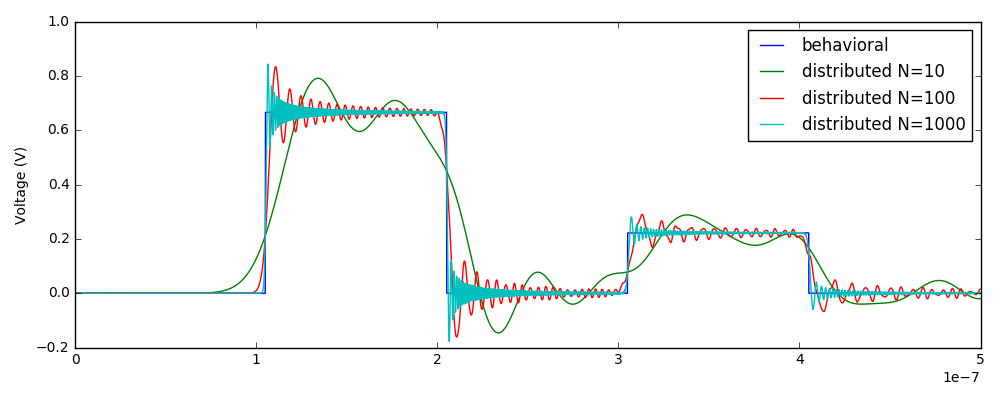
\includegraphics[width=0.3\textwidth]{src/2/figures/tline_comparison.pdf}
  \caption{Lumped versus two-port models comparison in simulation}
  \label{fig:lines-simulations}
\end{figure}


Overall, the behavioral model outperforms the distributed model for representing a perfect transmission line.
It reproduces exactly the 1ps risetime on the load in all configurations (Fig. \ref{fig:lines-simulations}).
The distributed model is either not as accurate or much slower to simulate.

\begin{table}[!h]
\centering
\begin{tabular}{@{}lllll@{}}
\toprule
amount N         &  10           & 100        &  1000      &   10000    \\ \midrule
simulation time  &  15 ms        & 170 ms     &  7.5 s     &   135 s    \\
increase ratio   &  -            & x10        &  x44       &   x18      \\
\bottomrule
\end{tabular}
\caption{Impact of the amount of unit elements on the simulation times}
\label{tab:tline-impact-simulation-time}
\end{table}

Autres elements, tels que elements passifs, protections esd, etc.

Application de la méthode sur un générateur TLP réel

% Illustrate the method with a practical case
The methodology described previous (section \ref{sec:esd-modeling}) is applied to the \gls{tlp} bench at NXP laboratory in Toulouse.
It is a good illustration on how to use the library of models for simulating a complete system.
Also, this particular testbench is widely used in NXP for characterizing and testing products.
The model described hereafter is used for instance to validate non-linear frequency model of passive devices.

% Describe the approach
To demonstrate its accuracy, the bench model is verified with an extensive simulation versus measurement comparison flow.
First, its behavior is measured under different loads and at different charging amplitudes.


\begin{figure}[!h]
  \centering
  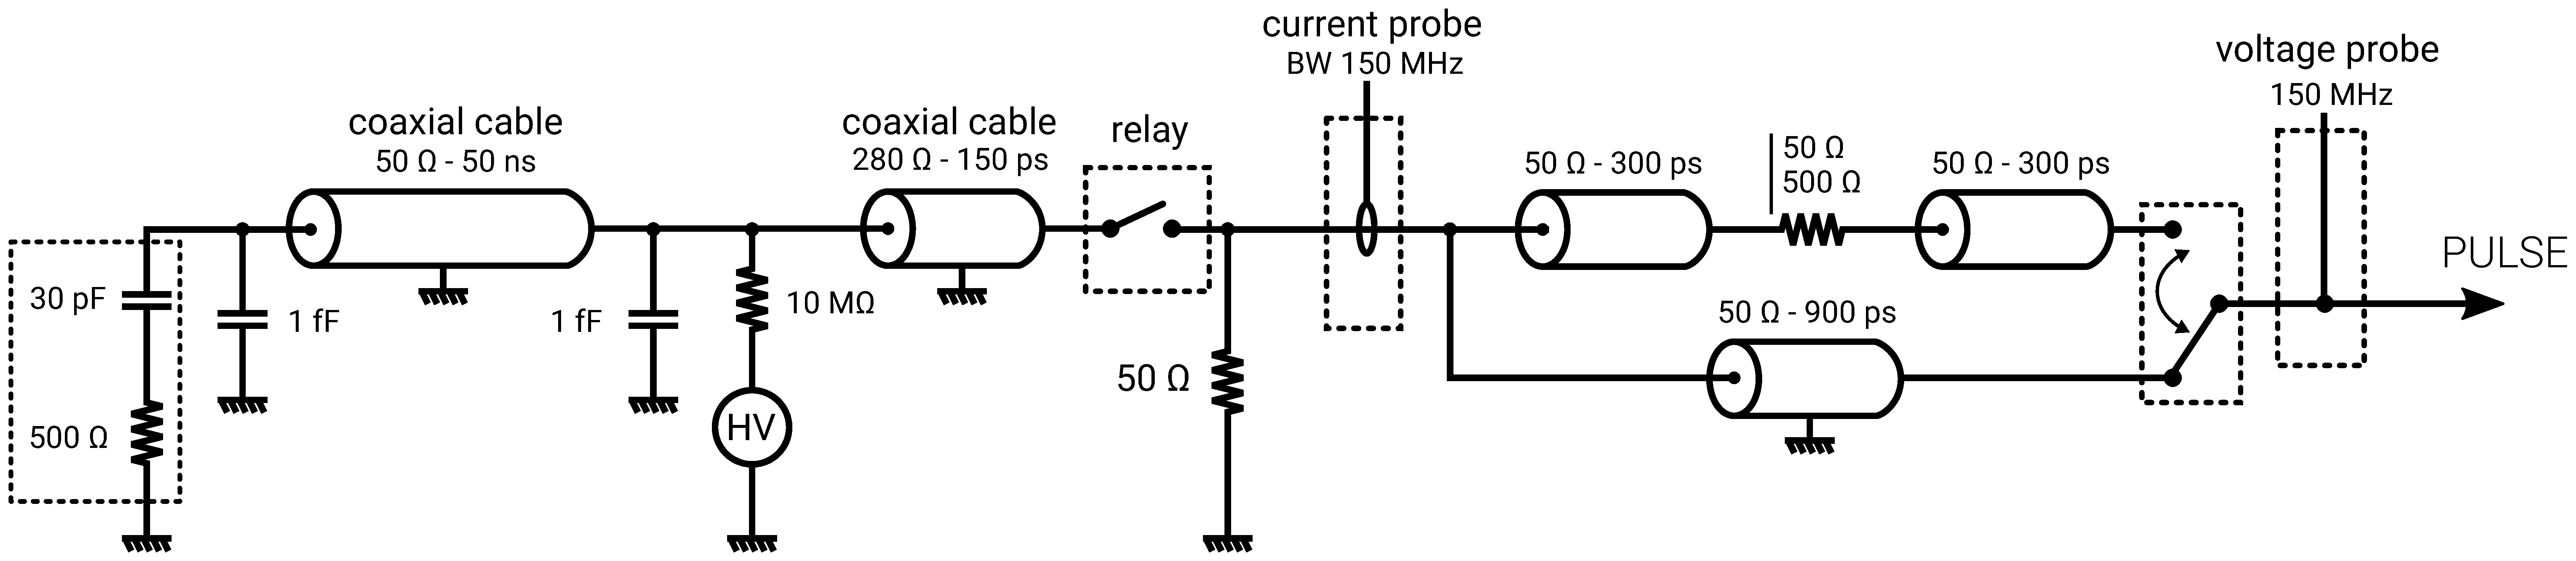
\includegraphics[width=\textwidth]{src/2/figures/complete_nxp_tlp_model.pdf}
  \caption{Complete model of NXP laboratory's TLP generator}
  \label{fig:complete-tlp-model}
\end{figure}

% Explain how the model, how it was constructed
The complete model is detailed in Fig. \ref{fig:complete-tlp-model}.
Similarly to all TLPs, the principle of operation is rather straightforward.
Initially, the relay is left open while the 50ns coaxial cable on the left is being charged by the high voltage \gls{dc} supply.
The 10 M\textOmega{} resistor ensures that the cable charges slowly to avoid oscillations, and isolates the high voltage supply from the pulse.
The two $1 fF$ capacitors placed at each end of the discharge cable help the simulator respect the initial condition for the charging voltage.
The cable is pre-charged to accelerate the simulation.
After the relay, a 50 \textOmega{} resistor can be found, intended as an attenuator.
Despite having a value of 50\textOmega{} like the coaxial cables, this resistor creates an impedance mismatch.
It is the perfect illustration of a small element that is easily missed out but impacts waveforms a lot.
A current probe is connected immediately after the attenuator, and a voltage probe is connected at the output of the generator.
Position of the probes are important as well, to reproduce the timeshift between them.
The short transmission line represented by 150 ps coaxial cables is a piece of barenaked wires.
It creates impedance mismatches because it has an estimated characteristic impedance of 280 \textOmega{}.
Finally, two discharge paths are possible inside the generator depending on the configuration of the switch on the output.
The direct path is at the bottom, where the pulse goes straight out from the generator.
The top path provides a series resistance that limits the discharge current.

% Detail a first comparison with 25 ohms
A first comparison between measurement and simulation is given in Fig. \ref{fig:comparison-tlp-load}.
With a 25\textOmega{} resistor and a charging voltage of 500V, 4.5A (I\textsubscript{TLP}) of current and 125mV (V\textsubscript{TLP}) are recorded.
The ratio of V\textsubscript{TLP}/I\textsubscript{TLP} between 40 ns to 100 ns is equal to 25\textOmega{} as expected.
Until 220 ns, both curves match closely.
After this time, some differences appear due to the bouncing back and forth of the pulse inside the system, and the accumulation of model errors.
However, most ESD investigations focus on the main part of the discharge under 120 ns.

\begin{figure}[!h]
  \centering
  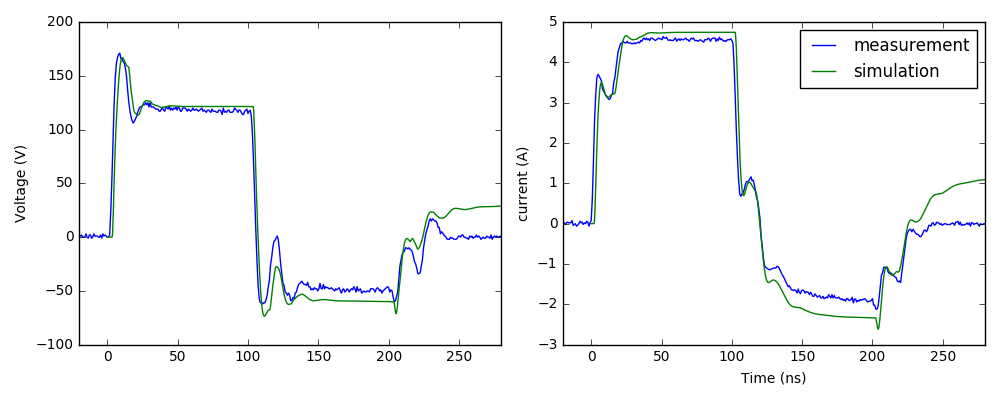
\includegraphics[width=\textwidth]{src/2/figures/tlp_comparison_R25_500V.png}
  \caption{Voltage and current waveforms comparison - 500 V charging voltage on 25\textOmega{}}
  \label{fig:comparison-tlp-load}
\end{figure}

% More validations in Annex
More simulation and validation curves are provided in Annex \ref{apx:tlp-validation-curves}, for different loads and amplitudes.
The goal of all those validation is to verify the model at both nominal and boundary conditions.
Overall, the model is good and fits very well the measurements, demonstrating the validity of the modelling method.

\section{Dévelopement d'un générateur TLP modifié}

Pour la génération de pulse HMM

%TODO: Simplifier
% TLP is a great tool for esd analysis
Throughout this document and in the \gls{esd} field in general, the \gls{tlp} generator is used extensively as a characterization and testing tool.
Amoung its many advantages, it generates very clean and controllable pulses in a shielded environment.
It has also proven to be a great tool for studying, among other things, the behavior of silicon-level devices.
% But ESD gun is required.
Nevertheless, \gls{esd-gun} testing remains the mandatory requirement defined by customers for product qualification.
\gls{tlp} testing alone is not a sufficient proof for customers that the integrated circuit can survive the harsh real environment, especially for automotive applications.
Several \gls{esd-gun} standards exist, targeting qualification of devices against electro-static discharges.
The HMM specification \cite{hmm}, the IEC 61000-4-2 standard \cite{iec61000-4-2} and the ISO 10605 standard \cite{iso10605} define the same \gls{esd} testing waveform, using the same discharge device, but with different application conditions.
Together, they cover a very large amount of tested devices from equipment, boards, and integrated circuit, in automotive and consumer fields.
The waveform common to those three standards (Fig. \ref{fig:hmm-waveform}) is virtually the most widely used pulse for ESD qualification.

\gls{tlp} cannot be used as a drop-in replacement to \gls{esd} gun for qualification.
A compromise can be found by modifying a \gls{tlp} generator to produce the gun waveform, but in a shielded, well-controlled, and reproducible environment.
This approach has been explored in the past by E. Grund \cite{iec61000-tlp} and Y. Cao \cite{tlp-based-hmm}.

The TLP-HMM requires two additional modules to be connected at each extremity of a classic 100ns \gls{tlp}.
These modules are simply referred hereafter as the \textit{absorber} and the \textit{shaping filter} (Fig. \ref{fig:tlp_hmm_architecture}).
The principle of the TLP-HMM is to re-route parts of an incoming rectangular pulse into the ground.
The remaining current is injected on a 2\textOmega{} calibration resistor, resulting in the same waveform than expected by the standards.
The role of each module is detailed in the following sections.

\begin{figure}[!h]
  \centering
  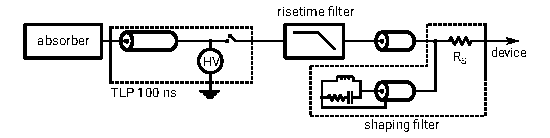
\includegraphics[width=0.9\textwidth]{src/5/figures/beges_tlp_hmm.pdf}
  \caption{TLP-HMM architecture}
  \label{fig:tlp_hmm_architecture}
\end{figure}


% Role of the shaping filter
The shaping filter (see Fig. \ref{fig:shaping_filter_example}) deviates a part of the incoming rectangular pulse into the grounded coaxial shielding.
It is constituted of five different elements, an RLC network, a delay cable and an injection resistor.
The capacitor C is separated from the main propagation path by a small transmission line of delay \textDelta{}t.


\begin{figure}[!h]
  \centering
  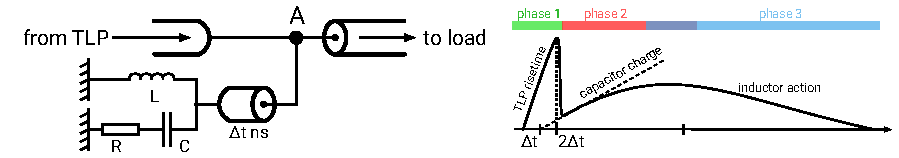
\includegraphics[width=0.98\textwidth]{src/5/figures/example_tlp_hmm.pdf}
  \caption{Shaping filter architecture and operation}
  \label{fig:shaping_filter_example}
\end{figure}

% Behavior of the filter - C
An example case is given to detail the behavior of the generator, with a focus on the shaping filter.
In phase 1 (graph on the right in Fig. \ref{fig:shaping_filter_example}), a \gls{tlp} is injected on the main line.
It reaches point A at $t=0$ and the voltage at A rises from 0 V.
The capacitor is still not visible from A and does not see the TLP rising edge yet.
At $t=\Delta t$, the pulse reaches the capacitor, which begins to charge.
This change in voltage and current in the capacitor branch is not visible immediately from point A until it propagates back.
Point A keeps rising with the TLP impulse until $t=2\Delta t$.
At this moment, potential at point A falls almost immediately to 0V, because the capacitor is drawing all the current, and its potential is low.
This results in the generation of the first peak.
The peak width is approximately $2\Delta t$.

% Behavior of L
In phase 2, the capacitor keeps charging, the potential at point A rises and the current drawn by the capacitor decreases.
Slowly, the inductor L connected in parallel starts drawing some current.
At some point between phase 2 and 3, the inductor current becomes equal to the capacitor current, and the capacitor ceases to charge.
The capacitor starts discharging through the inductor.
During phase 3, the inductor draws all the current and brings the voltage at A down to 0V.
The result of this combined action generates the characteristic slow slope of the HMM waveform.

% Behavior of R
The resistor R creates an voltage offset at $t=2\Delta t$.
It is used to match better the standardized waveform, which also has a superior to zero value after the first peak.

% Tuning the peak width
The peak width can be tuned by increasing or decreasing the length of the delay cable $t=\Delta t$.
The peak width is approximately equal to $t=2\Delta t$.

% Tuning the peak risetime
The peak risetime is enforced by the \gls{tlp} risetime filter.
A 1ns risetime filter provides the correct risetime to be compliant with the standards.
Several risetime filters implementations suitable for TLP generators have been described in \cite{gaussian-lpf,cao-risetime-filter}.
Matched risetime filters have the particularity to work by absorption, rather than rejection.
Most filters prevent high-frequency signals to propagate further into a system by reflecting them back.
Risetime filters on the other hand route high-frequencies into the ground of the system, which leaves the main signal line free of noise.

% Introduce the design
The exact schematic of the shaping filter is given in Fig. \ref{fig:shaping_filter_schematic}.
Capacitances are distributed to reduce parasitic inductances.
The inductances have also been distributed to increase the maximum total current that can be absorbed.
The PCB (Fig. \ref{pic:shaping_filter_assembled}) has a ground plane, and the central line is 50\textOmega{} matched.
Overall, its dimensions must be kept as small as possible to reduce the impact of delays.

\begin{figure}[!h]
  \centering
  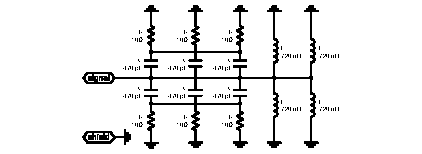
\includegraphics[width=0.9\textwidth]{src/5/figures/shaping_filter_schematic.pdf}
  \caption{shaping-filter schematic}
  \label{fig:shaping_filter_schematic}
\end{figure}

Near the end of the HMM waveform, the inductor is drawing almost all the incoming \gls{TLP} current.
After 100ns, the current injected by the TLP into the shaping filter and the \gls{dut} becomes null because the cable is completely discharged.
However, the current inside the inductor cannot be stopped instantly.
Without the absorber, the inductor would keep absorbing a non-zero current after the TLP pulse, drawing a negative potential at point A.
To avoid this phenomenom, the absorber completely filters the TLP falling edge at the end of the pulse.
This way, the current through the inductor is softly brought back to 0 by the absorber, effectively eliminating the negative voltage issue.
It also acts as a matched termination for transient events, which is great to eliminate reflections and prevent ringing oscillations.

The schematic of the absorber is given Fig. \ref{fig:absorber_schematic}

\begin{figure}[!h]
  \centering
  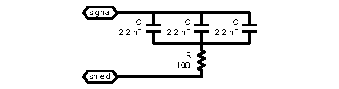
\includegraphics[width=0.7\textwidth]{src/5/figures/absorber_schematic.pdf}
  \caption{absorber schematic}
  \label{fig:absorber_schematic}
\end{figure}

The measured and simulated waveforms are given in Fig. \ref{fig:tlp_hmm_waveforms}.
Measured currents at 30ns and 60ns are within the 30\% tolerance of the standard (see Table \ref{tab:mes-sim-std-currents}).
The measured peak current is a bit lower (110 mA short of minimum margin) than standard value.
This is easily corrected on the TLP by adding a small positive offset to the charging voltage.

\begin{figure}[!h]
  \centering
  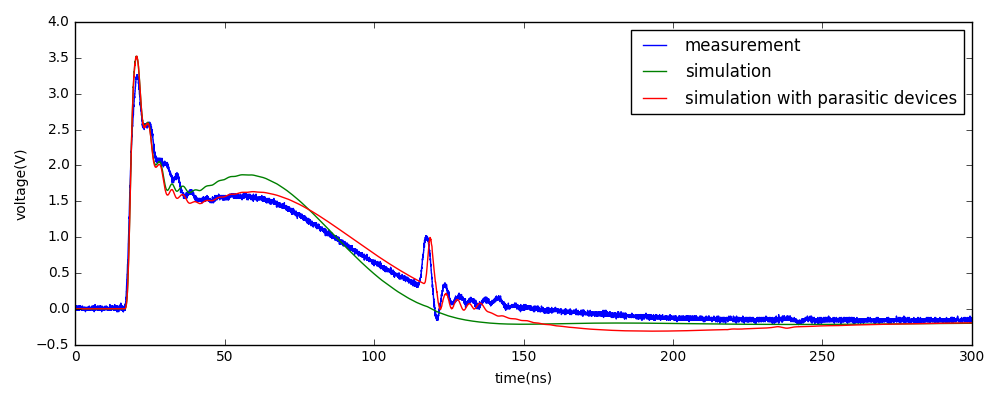
\includegraphics[width=0.95\textwidth]{src/5/figures/tlp_hmm_waveforms.png}
  \caption{Measurement versus simulation of a 250V TLP-HMM (equivalent 1kV HMM) on 2\textOmega{}}
  \label{fig:tlp_hmm_waveforms}
\end{figure}

% Analyse the curve
Overall, simulation and measurement correlate quite well.
There is a small difference for the slopes between 40ns and 150ns.
Investigation showed this difference comes from the shaping filter, and its inductances in particular.
Their frequency behavior is not as good as expected, and having four inductances in parallel increases further this issue.
Indeed, in this configuration parasitic capacitance of inductors are connected in parallel.
They add up together, leading to a large total parasitic value and degraded frequency behavior.
For the next iteration of the shaping filter, a single RF inductor should be used instead.


% Conclusion regarding TLP-HMM
In this section, a new alternative for generating HMM compliant waveforms using a TLP was presented.
The generator works correctly and has proven quite robust against ringing oscillations and parasitic disturbances.
The generated waveform passes HMM, IEC 61000-4-2 and ISO-10605 requirements.

% Limitations of the TLP-HMM
A prototype has been constructed to enable initial testing and evaluation of the system.
The design must be improved to reduce the impact of parasitic devices.
Also, higher charging voltages must be supported for the generator to inject larger amount of currents.
It is currently not enough to break ESD protections that withstand above 4A of transient current.
There are many challenges to be solved in order to build a TLP able to charge at 8kV and beyond.
For instance, the risetime filters are not able to sustain such elevated voltages and customs filters are probably required.

\section{Méthode de traitement de capteurs de courant on-chip}

% Introduction
Near-field scan has been presented previously in \ref{sec:near-field-scan}.
Using this technique it is possible to measure maps of electric or magnetic field above a device.
While those maps already provide interesting information, to locate sources of RF noise for instance, it is interesting to post-process them in order to get voltages and currents inside the measured circuit.
In this section, two different methods are described for reconstructing the original current from a near-field magnetic measurement.
Each method requires a preliminary characterization of the probe.
Near-field scanners were extensively studied in \cite{near-field-scan, phd-monnereau}.

% What is the output voltage that is measured
It is shown in \cite{near-field-scan} that the measured voltage of near-field magnetic probe is proportional to the time derivative of the measured and coupled current.
In the next part of this analyis, the sensor voltage is denoted V\textsubscript{sensor} and the original current I\textsubscript{TLP}.

it is possible to express I\textsubscript{TLP} as a function of the measured sensor voltage V\textsubscript{sensor}.
This is expressed in Eq. \ref{eq:nfs-rel2}.
The offset $A$ is the result of the integration.

\begin{equation}
I_{TLP}(t) = \frac{1}{G}\int V_{sensor}(t) \mathrm{d}t + A
\label{eq:nfs-rel2}
\end{equation}

% How to determine 1/G and A
Both constants $1/G$ and $A$ are determined experimentally with a preliminary calibration.
Once calculated, both factors are estimated to remain constant and can be reused in other measurements.

% Talk about calibration setup
On silicon, one of the sensors is dedicated to the calibration phase.
The setup is given in Fig. \ref{fig:calibration-sensor}.
The input of the sensor is represented by ports S1 and S2.
A square impulse of 1V amplitude generated by a 100ns wide TLP with a risetime of 8ns is injected between the two input pins.
The response V\textsubscript{sensor} is measured with a 2GHz bandwith 10GS/s oscilloscope in differential input connected between C1 and C2.

\begin{figure}[!h]
  \centering
  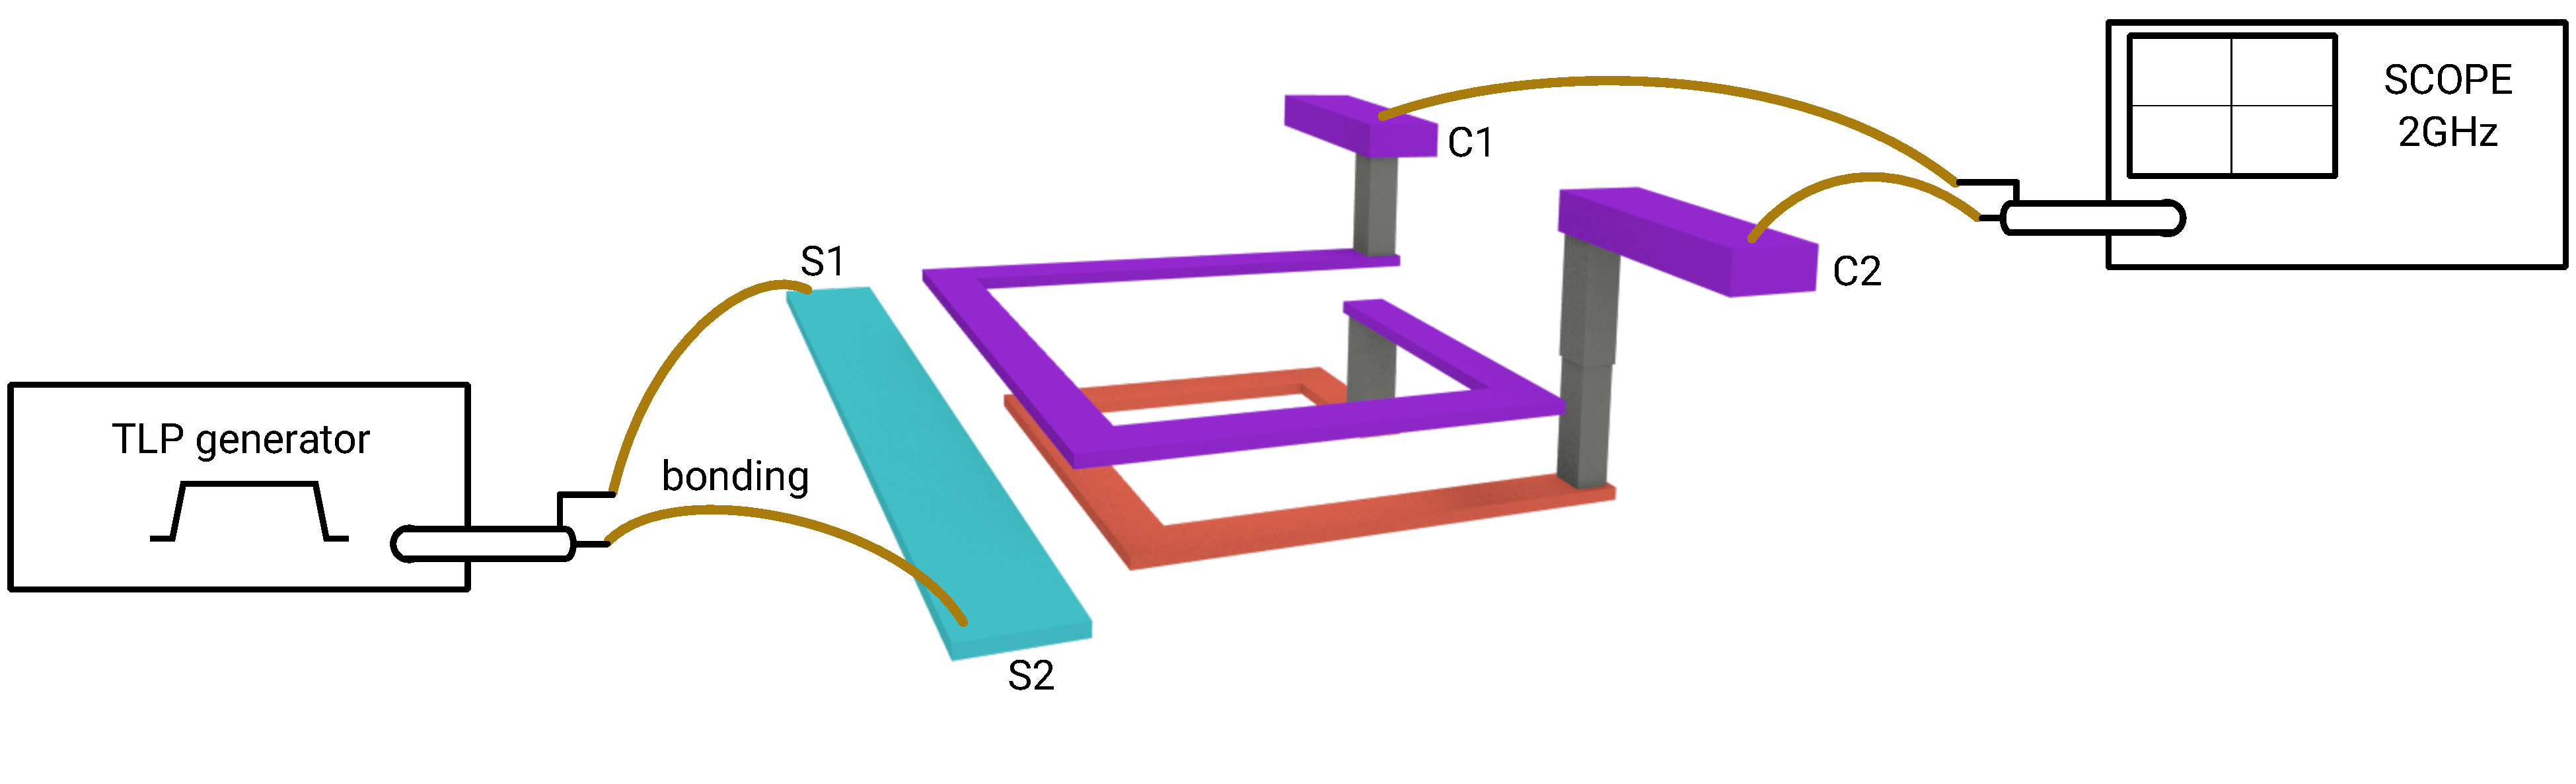
\includegraphics[width=0.9\textwidth]{src/3/figures/sensor_measurement_setup.pdf}
  \caption{Calibration sensor setup for time-domain method}
  \label{fig:calibration-sensor}
\end{figure}

% Explain the measurements
I\textsubscript{TLP} and V\textsubscript{sensor} waveforms are recorded during calibration (see Fig. \ref{fig:measurement-nfs}).
The top curve represents the input (I\textsubscript{TLP}) and the bottom curve the output (V\textsubscript{sensor}).

\begin{figure}[!h]
  \centering
  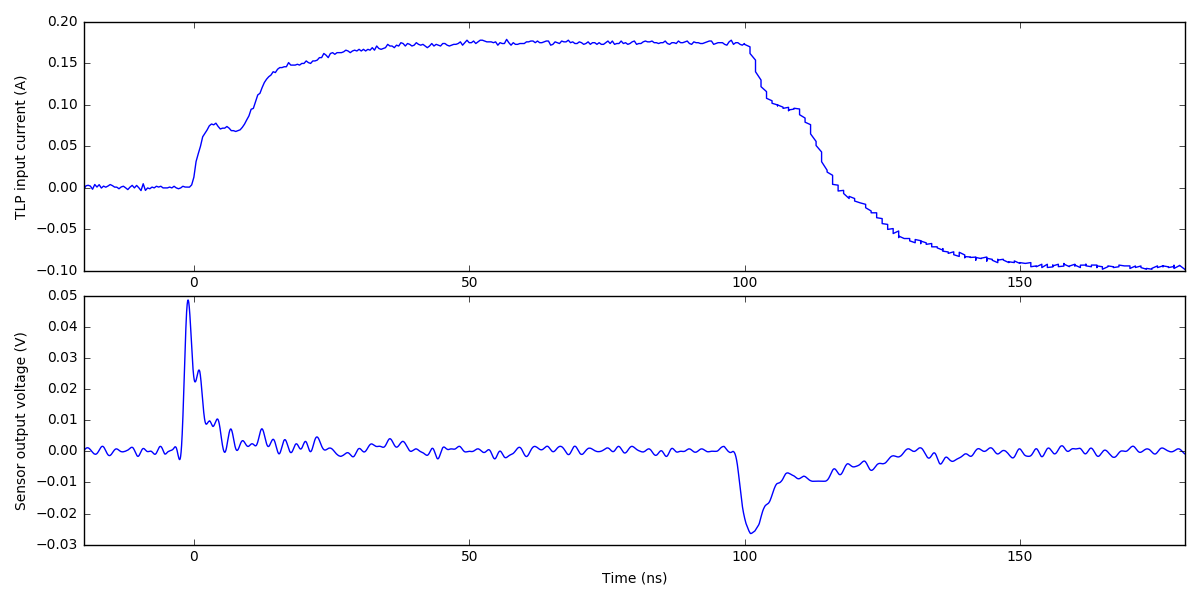
\includegraphics[width=0.95\textwidth]{src/3/figures/measured_waveform.png}
  \caption{Measured voltage waveform}
  \label{fig:measurement-nfs}
\end{figure}

% Integration method
With those measurements, $1/G$ and $A$ are determined experimentally.
Both values were estimated at $1/G = 8.10^8$ and $A = -V_{TLP}(t = 0)$.

% Intro & Characterization
The frequency-domain method post-processes the V\textsubscript{sensor} waveform using the sensor's frequency response.
The characterization is conducted with the calibration sensor, using a \gls{vna}.
The calibration setup is similar to the time-domain method.
It is given in Fig. \ref{fig:calibration-sensor-rf}.

\begin{figure}[!h]
  \centering
  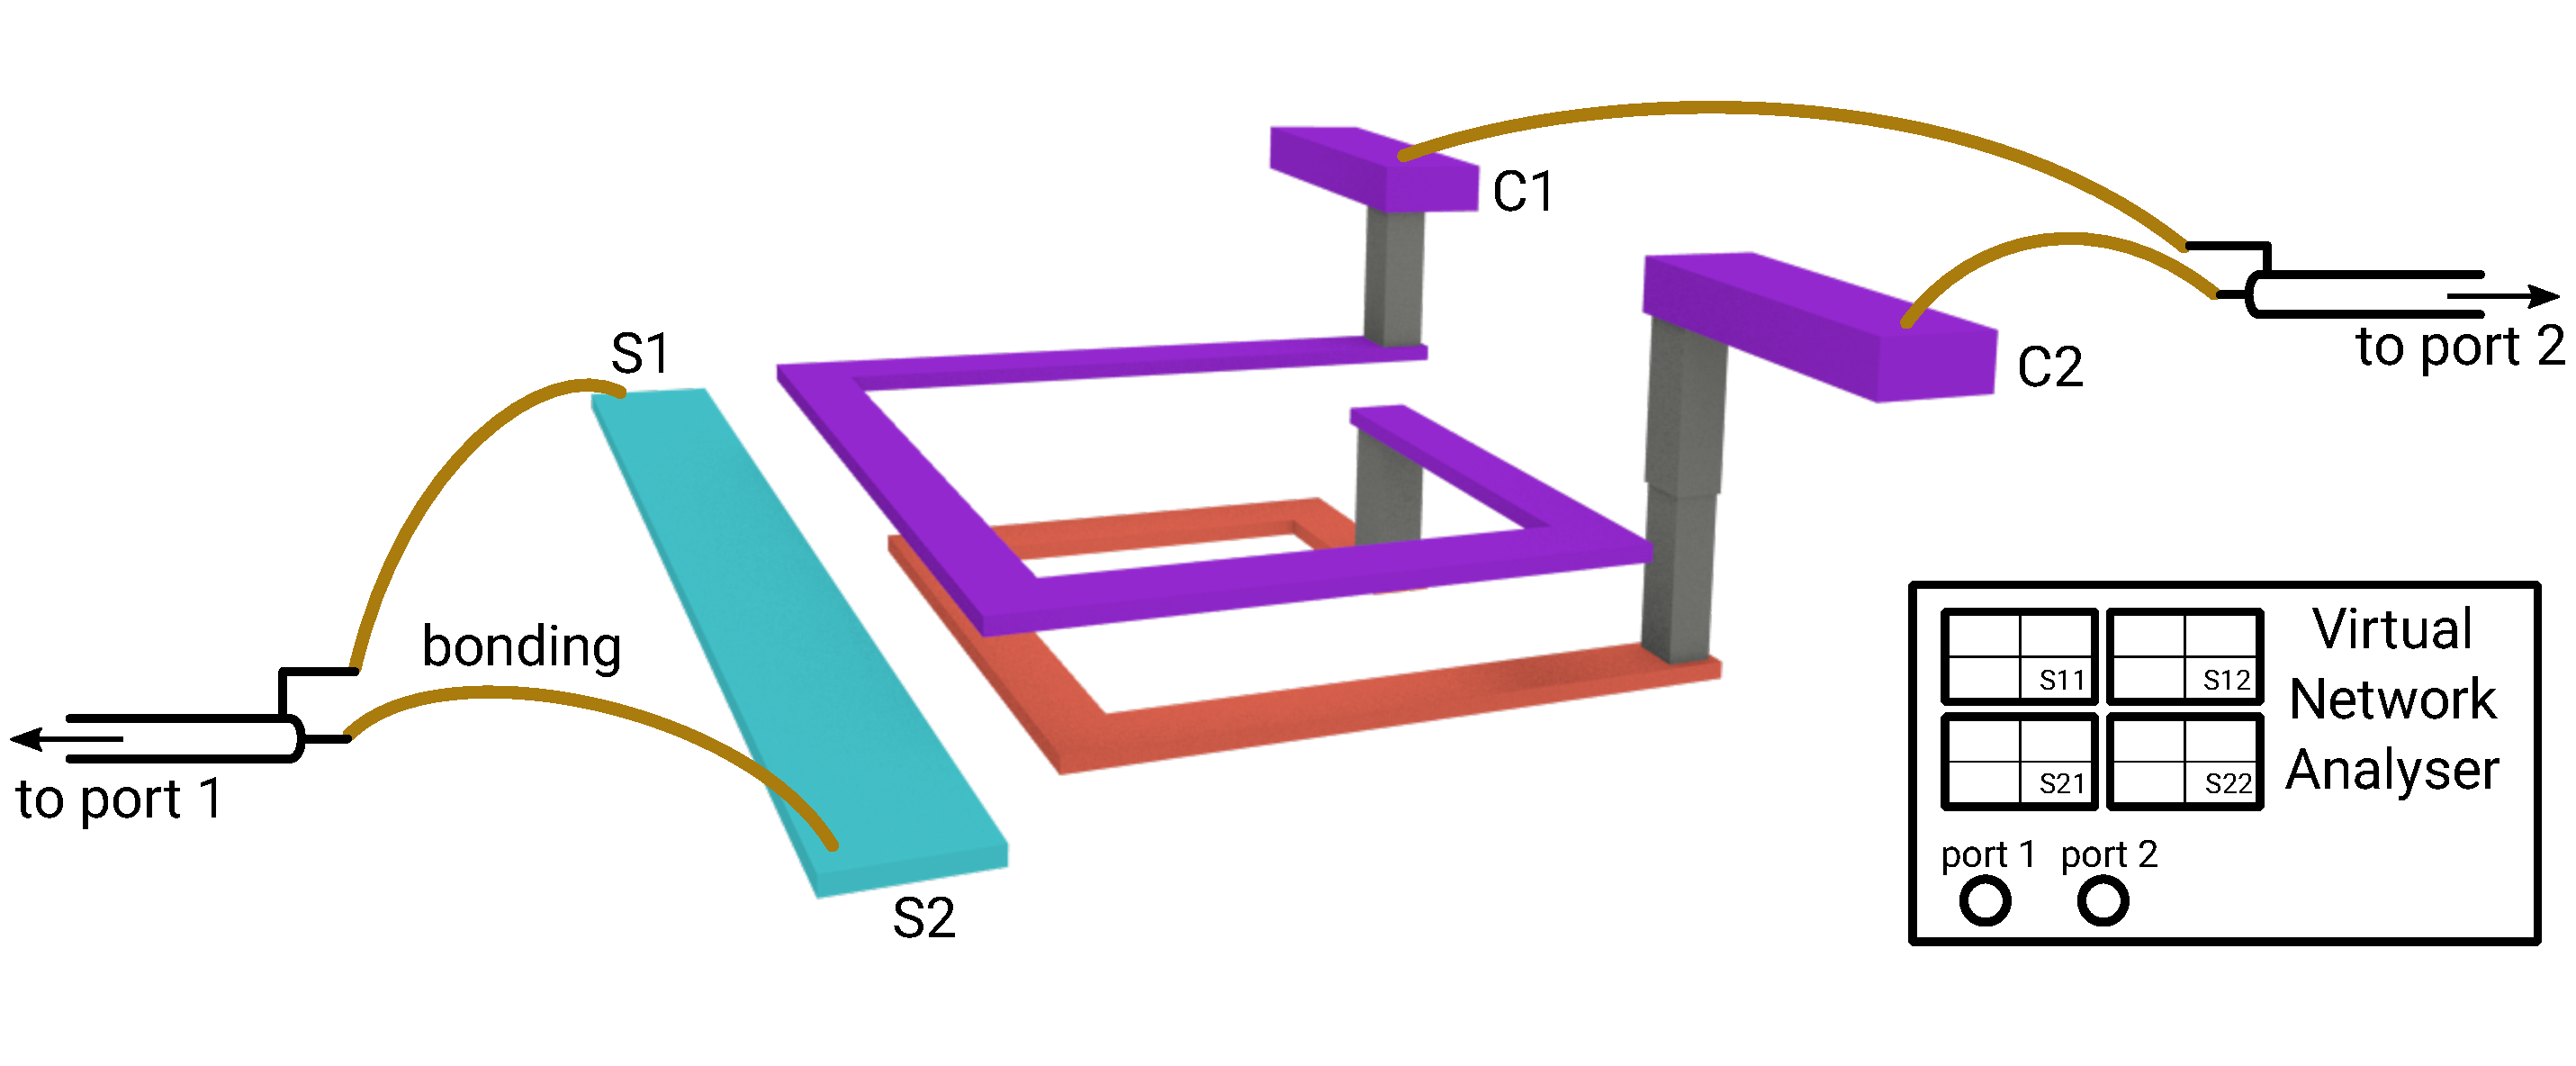
\includegraphics[width=0.9\textwidth]{src/3/figures/sensor_measurement_setup_rf.pdf}
  \caption{Calibration sensor setup for time-domain method}
  \label{fig:calibration-sensor-rf}
\end{figure}

% Detail characterization
The \gls{sparams} measurements of the sensor are given in Fig. \ref{fig:sensor-response}.
$S11$ is the reflected power at port 1.
$S21$ is the transmitted power between port 1 and port 2, and $S12$ is the transmitted power between port 2 to 1.
In theory, $S12$ is identical to $S21$ for symetrical 2-port devices.
$S22$ is the reflected power from the output, which is not relevant for this study.

\begin{figure}[!h]
  \centering
  \includegraphics[width=0.9\textwidth]{src/3/figures/sensor_freq_response.png}
  \caption{Sensor frequency response}
  \label{fig:sensor-response}
\end{figure}

% Analyse the response
It was suspected previously that the sensor's response is not constant versus frequency.
The \gls{sparams} measurement confirms it, showing a sensor bandwidth of about 300MHz.

% Talk about S11
S11 shows a resonance of -43.9 dB at 1.15 GHz.
It corresponds to a frequency where insertion losses become very small.
However, this peak is not visible on the transmitted coefficient $S12$ or $S21$.
It probably means that at this frequency, a part of the input power is dissipated by the device, either by the bonding or the sensor itself.


\begin{figure}[!h]
  \centering
  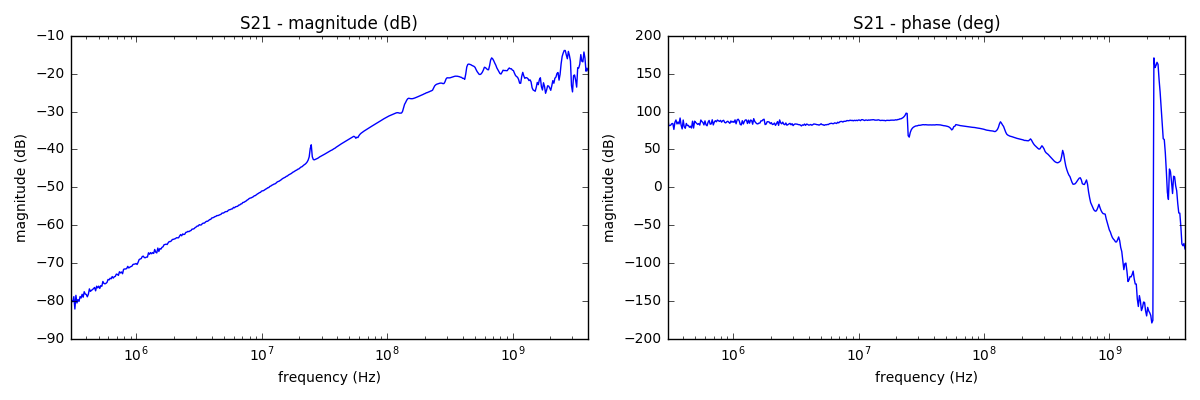
\includegraphics[width=0.9\textwidth]{src/3/figures/s21_freq_response.png}
  \caption{Sensor frequency response - complex S21 (magnitude and phase)}
  \label{fig:s21-response-complex}
\end{figure}

\begin{figure}[!h]
  \centering
  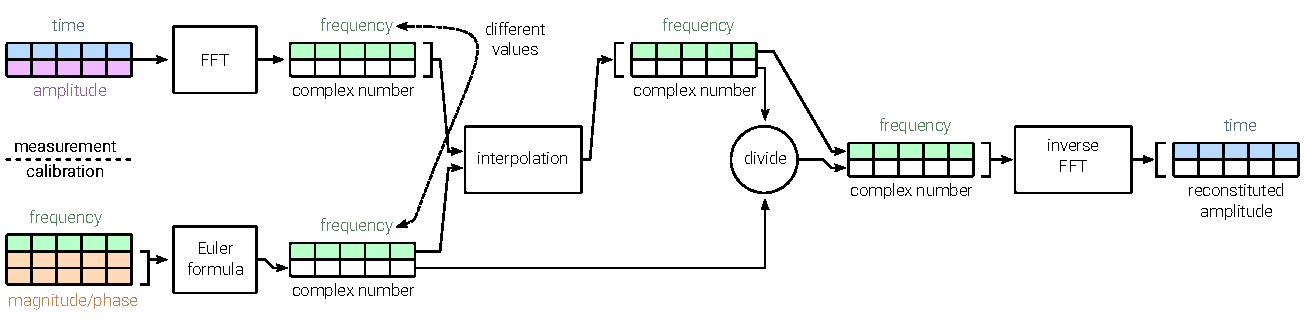
\includegraphics[width=\textwidth]{src/3/figures/frequency_post_process_flow.pdf}
  \caption{Post-processing pipeline}
  \label{fig:postprocess-nfs-pipeline}
\end{figure}

% The algorithm
The post-processing method is detailled in Fig. \ref{fig:postprocess-nfs-pipeline}.
The measurement data in the time-domain is converted to the frequency domain using \gls{fft}.
The ouptut array associates to each frequency point a complex number.
An example is given in Table \ref{tab:complex-fft}.

\begin{table}[!h]
  \centering
  \begin{tabular}{@{}lllll@{}}
  \toprule
  frequencies (Hz)        & complex value                \\ \midrule
  1.0*10^6                & 0.33 + i0.2                  \\
  2.0*10^6                & 0.46 - i1.2                  \\
  etc.                    & etc.                         \\ \bottomrule
  \end{tabular}
  \caption{Structure for the result of (complex) FFT}
  \label{tab:complex-fft}
\end{table}

On the other hand, the S21 calibration data associates a phase and magnitude to each frequency point.
An example is given with Table \ref{tab:sparams}.
Using Euleur formula (Eq. \ref{eq:to-complex}), magnitude and phase are converted to a complex number.

\begin{table}[!h]
  \centering
  \begin{tabular}{@{}lllll@{}}
  \toprule
  frequencies (Hz)          & magnitude (dB)         & phase (rad)     \\ \midrule
  1.5*10^6                  & -10                    & 1.23            \\
  2.5*10^6                  & -12                    & 0.12            \\
  etc.                      & etc.                   & etc             \\ \bottomrule
  \end{tabular}
  \caption{Structure for the S-parameter measurement}
  \label{tab:sparams}
\end{table}

\begin{equation} \label{eq:to-complex}
  S21_{complex} = 10^{\frac{magnitude}{20}} * (\cos(phase) + i*\sin(phase))
\end{equation}

% Interpolation step
After these two operations, both data are in the frequency domain.
Before moving forward in the processing, an interpolation step is required.
Indeed, the frequency points between the measurement and the calibration do not match.
For the next part of the algorithm, they need to be identical.
In this case study, a linear interpolation is employed on the measurement data to align it on the characterization.
It is possible that this kind of interpolation is not ideal.
The impact of the interpolation on the results has not been studied yet but it should be done in a future work.

% Compensation
Afterwards, the measurement data is compensated by the characterization data of the sensor.
This is done by dividing each complex value of the measurement by the complex value of the sensor.

% Inverse FFT
Finally, the inverse \gls{fft} of the compensated data is calculated to bring back the waveform into the time-domain.
The resulting waveform is compared to the original and the integration method in Fig. \ref{fig:freq-domain-reconstructed}.
Overall, the results are similar between the time-domain and frequency-domain reconstitutions.
The frequency domain seems to have more dynamic behavior, because it looks like it is reproducing rising and falling edges better.
However, they have both large errors after the pulse and fail to reproduce the reflected wave.
There is a lot of room for improvement for each method, such as increasing the measurement frequency, and using techniques like zero-padding before performing \gls{fft} and taking dissipated power into account.

\begin{figure}[!h]
  \centering
  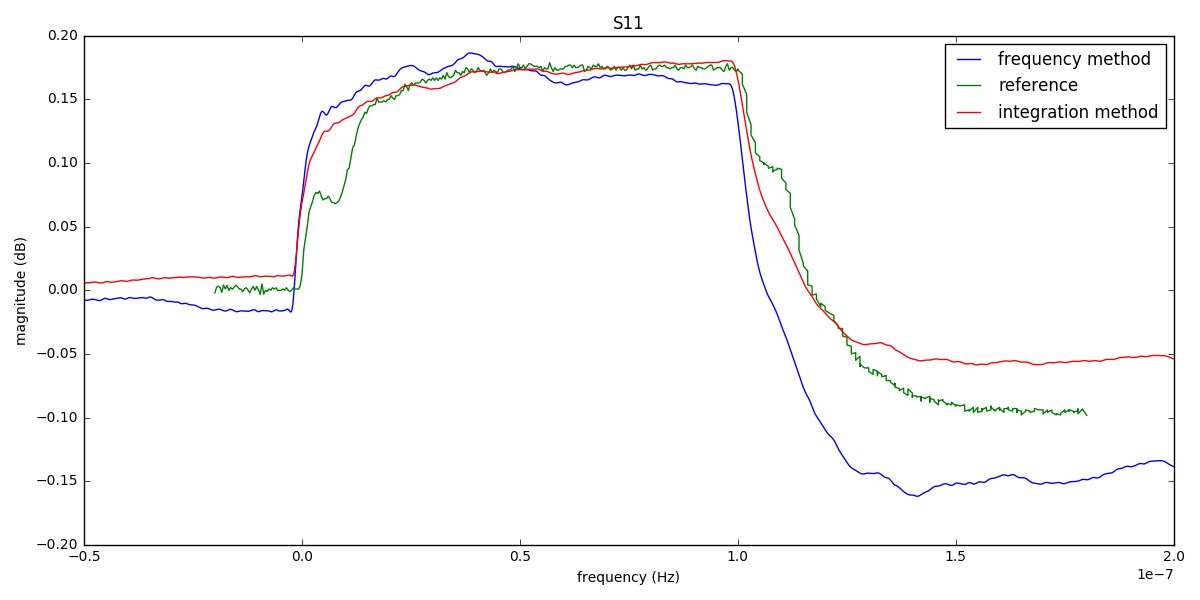
\includegraphics[width=0.9\textwidth]{src/3/figures/final_comparison_reconstructions.png}
  \caption{Reference current waveform versus frequency-domain and time-domain reconstructions}
  \label{fig:freq-domain-reconstructed}
\end{figure}
